\chapter{Bitcoin peer-to-peer network}
\label{sec:netintro}

Bitcoin nodes form an overlay network and communicate through a specific application-level protocol.

The topology of the Bitcoin network is unknown, but is generally considered to be structured as a random graph. Topology information is kept hidden as it can enable attacks on privacy~\cite{biryukov2014deanonymisation}. The interested reader can find more in the work of Deshpande et al.~\cite{Deshpande2018BTCmapMB}.\par

The Bitcoin network is extremely diverse as different kind of nodes can join. The Bitcoin Reference Client developed by Nakatomo is provided with a \textit{wallet}, which is an applicative module for payments, has a network interface, stores all the blockchain and is a miner at the same time. These can be defined as \textit{full nodes}.

Nonetheless, not all nodes may want to store the entire blockchain or mine. Some miners often store only the headers of the blockchain in order to save space. Other users install only the wallet and do not take part in mining and verification at all.

An important exception are the unreachable nodes. These nodes work behind a NAT and often mine together in \textit{mining pools}. A central server manages all the incoming traffic and shares the mining rewards among pool workers.

Nowadays most of the users that want to have a revenue from mining work in pools and therefore the number of the reachable nodes is not representative of the dimension of the network. In general the number of reachable nodes is always around ten thousand~\cite{totknownfullnodes}.\par

In this work only full nodes are considered as they are the ones that have an active role on the network.

The following chapters provide a complete overview of the Bitcoin protocol.

\section{Connection and peer discovery}\label{sec:peerdisc}
In order to establish a connection two peers need to exchange version messages over an unencrypted TCP channel in a handshake fashion as shown in Fig.~\ref{fig:btcconn}. The node that first sends a \texttt{version} message establishes an \emph{outgoing connection}. The receiving node sets up an \emph{ingoing connection} instead. Once the handshake is completed the connection is fully set up.

\begin{figure}[h]
	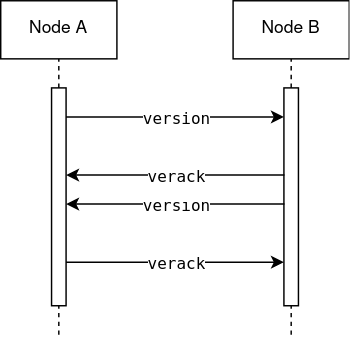
\includegraphics[width=.45\textwidth]{pict/BTCconnection.png}
	\centering
	\caption{Peers connection handshake}
	\label{fig:btcconn}
\end{figure}

Each node is capable to establish up to 8 outgoing connections and 117 ingoing connections, for a total of 125 connections. In order to keep its connections active, each peer sends a message to each neighbour at least once every thirty minutes. If more than ninety minutes pass without receiving anything from a neighbour, the connection is dropped.

Each node always tries to keep eight outgoing connections active, therefore, upon dropping an outgoing connection, a node tries to connect to another address in its peer cache.\par

Nodes on fresh bootstrap make use of hardcoded \emph{DNS seeds} as their first mean to discover other peers. DNS seed servers are maintained by community members and provide clients with a list of addresses that can be either dynamically gathered through a periodic scan of the network or manually updated by server administrators.

As a fallback option the user is able to specify through command line a list of addresses the client can connect to. Were both these two options to fail the client has a hardcoded list of peers it can directly connect to, though this is considered the last resort for bootstrapping peers.\par

Nodes at startup that were previously on the network shall first lookup peer names in their local address database, implemented as "peer.dat". The database contains the address of each peer the node has come to know during its lifetime in the network.

If the node has disconnected for a time too long, many of the addresses in the database may have become outdated or unreachable. A node that cannot connect to any address in the peer database, or has spent up to eleven seconds trying to connect unsuccessfully to at least one of the peers in the database, behaves as on fresh bootstrap and resolves to query a DNS first.

The use of a local address database, also called \emph{peer cache}, provides reconnecting peers a fully-decentralized way to join the network and is the first line of defence against \emph{fake bootstrap attacks}; the topic along with other security concerns is discussed in Chapter~\ref{sec:netsec}.\par

Peer discovery after the first connection of a node is carried on through the exchange of \texttt{addr} messages containing the address and port number of other peers in the network~\cite{protocoldoc}~\cite{devguidep2p}.

On connection set up the two nodes exchange \texttt{addr} messages, as shown in \emph{Fig.~\ref{fig:addr}}, providing each other with addresses from their local peer database.

On top of that, every twenty-four hours each node advertises itself on the network with an \texttt{addr} message containing only its own address.

\begin{figure}[h]
	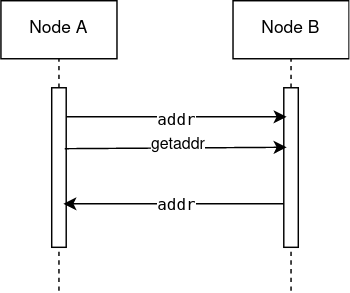
\includegraphics[width=.45\textwidth]{pict/BTCaddr.png}
	\centering
	\caption{Addresses exchange upon connection}
	\label{fig:addr}
\end{figure}

\texttt{addr} messages can contain at most one thousand addresses; additionally those containing ten or fewer addresses are relayed. This behaviour contributes to the gossiping of self-advertisement messages even though messages are relayed only to a small subset of neighbours, namely to a couple of peers.

\section{Peer database structure}\label{sec:cachestruct}
The local peer database or cache serves the purpose of storing the addresses a node has come to know from \texttt{addr} messages and DNS seeds. The database is constituted of the \texttt{new} and the \texttt{tried} tables.

The \texttt{tried} table contains addresses of peers with whom the node has successfully established a connection in the past. It consists of 64 buckets that can store up to 64 unique addresses. Buckets are selected through a hash on the IP address.

The \texttt{new} table contains the addresses the node has not connected to and is therefore larger: it has 256 buckets of 64 addresses each.

Peer caches have been widely implemented in distributed systems so far as they are a fast and fully-decentralized way to rejoin the network after a disconnection. They allow peer-to-peer systems to overcome major issues at bootstrap time, mainly related to the presence of a single point of failure, i.e. bootstrap servers. Furthermore, they are the most scalable and efficient solution when compared to other decentralized mechanisms such as \textit{address probing}~\cite{decentrbootstrapp2p}.

\section{Data dissemination}\label{sec:dissem}
Data is \texttt{gossiped} through the network. A gossip or \textit{epidemic} protocol is a communication paradigm for distributed systems where data is sent only to a subset of neighbours in order to reduce network traffic whilst still ensuring full coverage.

Nevertheless, no assumption can be made on the behaviour of nodes, therefore different nodes may implement different relay strategies.

Bitcoin Core simply broadcasts transactions and blocks to reduce their latency and keep local views consistent.

On top of that a simple strategy is adopted to try to enforce anonymity: it relays data with independent, exponential delays. Although, this policy has been proven extremely weak.

Various researches have proved that it is fairly easy for an adversary to deanonymize users~\cite{biryukov2014deanonymisation},~\cite{koshy2014deanon}. For this reason new dissemination protocols are now being adopted, first of which is \textit{Dandelion}. 

Dandelion has two distinct phases for dissemination: a \textit{stem} phase and a \textit{fluff} phase. During the stem phase the message is relayed multiple times to one neighbour only each time, so that the message creator is kept hidden. Once the stem phase ends, the data is normally broadcast in the network~\cite{dand}

Dropping a message during the stem phase loses the data completely, thus the protocol is extremely weak to malicious behaviour from neighbours, like block withholding (see Sections~\ref{sec:sybil}).

For this reason, \textit{Dandelion ++} was developed. In this version, honest nodes that forward data during the stem phase set a timer. If they do not see the forwarded message come back in fluff phase by the end of the timer, they broadcast the message themselves, forcing fluff phase~\cite{dandplus}.

With this simple change, Dandelion ++ greatly improves Dandelion robustness~\cite{lunes-dissemination}.\par

In this work, the tests are carried out using \textit{fixed probability} gossip, where a message is sent to each neighbour with a fixed probability, and Dandelion ++.